\documentclass[letterpaper]{article}
\usepackage[top=2cm, bottom=3.5cm, left=2.5cm, right=2.5cm]{geometry}
\usepackage{amsmath,amsthm,amssymb}
% Indicator function
\usepackage{bbm}
\usepackage{tikz}
\usepackage{enumitem}
\usepackage{booktabs}
\usepackage[T1]{fontenc}
\usepackage{indentfirst}

\usepackage{graphicx}
\usepackage{epstopdf}

% Bold vectors and matrices
\renewcommand{\aa}{\mathbf{a}}
\providecommand{\xx}{\mathbf{x}}
\providecommand{\yy}{\mathbf{y}}
\providecommand{\XX}{\mathbf{X}}
\providecommand{\YY}{\mathbf{Y}}
\providecommand{\vv}{\mathbf{v}}
\providecommand{\1}{\mathbf{1}}
\providecommand{\0}{\mathbf{0}}
\providecommand{\mA}{\mathbf{A}}
\providecommand{\mI}{\mathbf{I}}

\providecommand{\lin}[1]{\ensuremath{\left\langle #1 \right\rangle}}
\providecommand{\norm}[1]{\ensuremath{\left\lVert#1\right\rVert}}

%
% The following macro is used to generate the header.
%
\newcommand{\homework}[4]{
   \thispagestyle{plain}
   \newpage
   \noindent
   \begin{center}
   \framebox{
      \vbox{\vspace{2mm}
    \hbox to 6.28in { {\bf EE-556: Mathematics of Data \hfill Fall 2019} }
       \vspace{6mm}
       \hbox to 6.28in { {\Large \hfill Homework \##1 - Due date: #2\hfill} }
       \vspace{4mm}
       \hbox to 6.28in { {\hfill Student: #3} }
      \vspace{2mm}}
   }
   \end{center}
}

\renewcommand{\phi}{\varphi}
\renewcommand{\epsilon}{\varepsilon}

% Use these for theorems, lemmas, proofs, etc.
\newtheorem{proposition}{Proposition}
\newtheorem{theorem}{Theorem}
\newtheorem{corollary}{Corollary}
\newtheorem{lemma}{Lemma}
\newtheorem{claim}{Claim}
\newtheorem{remark}{Remark}
\newtheorem{definition}{Definition}
\newtheorem{fact}{Fact}
\newtheorem{assumption}{Assumption}

\DeclareMathOperator*{\argmin}{arg\,min}
\DeclareMathOperator*{\argmax}{arg\,max}
\newcommand{\mbeq}{\overset{!}{=}}
\newcommand{\E}{\mathbb{E}}
\newcommand{\vect}[1]{\boldsymbol{#1}}

% Use Small capitals like in problem statement
\usepackage{sectsty}
\renewcommand{\thesection}{\Roman{section}} 
\renewcommand{\thesubsection}{\Roman{subsection}}
\allsectionsfont{\mdseries\scshape}

\begin{document}
\homework{2}{15\textsuperscript{th} November 2019}{Oriol Barbany Mayor}

\subsection*{Problem 1 - Minimax problems and GANs}
\begin{enumerate}
    \item
    \begin{align}
        \nabla f(x, y) = 
        \begin{bmatrix}
            \frac{\partial}{\partial x} f(x, y) \\
            \frac{\partial}{\partial y} f(x, y)
        \end{bmatrix} = \begin{bmatrix}
            y \\
            x
        \end{bmatrix}
        \label{eq:grad}
    \end{align}
    
    The first order stationary points are $\{(x,y):\ \nabla f(x,y)=\0\}=(0,0)$, so there's actually only one of such.
    
    \begin{align}
        \nabla^2 f(x, y) = 
        \begin{bmatrix}
            \frac{\partial^2}{\partial x^2} f(x, y) & \frac{\partial^2}{\partial x\partial y} f(x, y) \\
            \frac{\partial^2}{\partial y \partial x} f(x, y) & \frac{\partial^2}{\partial y^2} f(x, y)
        \end{bmatrix} = 
        \begin{bmatrix}
            0 & 1 \\
            1 & 0
        \end{bmatrix}
    \end{align}
    
    The Hessian gives information about the type of first order stationary points. In this case, it has eigenvalues $\lambda = [0, 1]$ in all domain, so $(0,0)$ is a saddle point
    
    \item For $(x^*, y^*)=(0,0)$, it's trivial to see that $0=f(x^*, y^*)\geq f(x^*, y)=0$ and $0=f(x^*, y^*)\leq f(x, y^*)=0$, so indeed $(x^*, y^*)$ is a solution to the problem $\min_x \max_y f(x,y)$.
    
    \item The distance in L2-norm to the optimal solution in iteration $k+1$ is
    \begin{align}
        \norm{(x_{k+1},y_{k+1})-(0,0)}^2&:=\norm{(x_{k}-\gamma y_k,y_k-\gamma x_k)}^2:=x_k^2 - 2\gamma x_k y_k + \gamma^2 y_k + y_k^2 + 2\gamma y_k x_k + \gamma^2 x_k^2\\
        &=(1+\gamma^2)(x_k^2 + y_k^2) := (1+\gamma^2) \norm{(x_k,y_k)}^2=(1+\gamma^2)^{k+1}\norm{(x_0,y_0)}^2
    \end{align}
    so if $(x_0,y_0)\neq \0$, the iterates diverge as $\mathcal{O}((1+\gamma^2)^k)$.
    \item 
    \begin{align}
        |f(\xx) - f(\yy)| = |\vv^T(\xx - \yy)| := |\lin{\xx - \yy, \vv^*}| \leq \norm{\vv} \norm{\xx - \yy} := B \norm{\xx - \yy}
    \end{align}
    where the inequality follows from Cauchy-Schwarz. So the set of functions that are $B-$Lipschitz with $B\leq 1$ is $\{f \in\mathcal{F}: \ \sqrt{v_1^2 + v_2^2} \leq 1\}$. 
    
    \item Note that in order to enforce that a function $f\in \mathcal{F}$ is $1-$Lipschitz, it's enough to normalize its vector $\vv$ so as it has unit norm, i.e. $\vv \leftarrow \frac{\vv}{\norm{\vv}}$.
    \item 
    The performance of the simultaneous and alternating updates is similar. The estimates at some iterations for this latter approach can be seen in Figure \ref{fig:gan}. Its oscillatory behavior is discussed in the last section of this exercise.
    \begin{figure}
        \centering
        \begin{minipage}{.3\textwidth}
         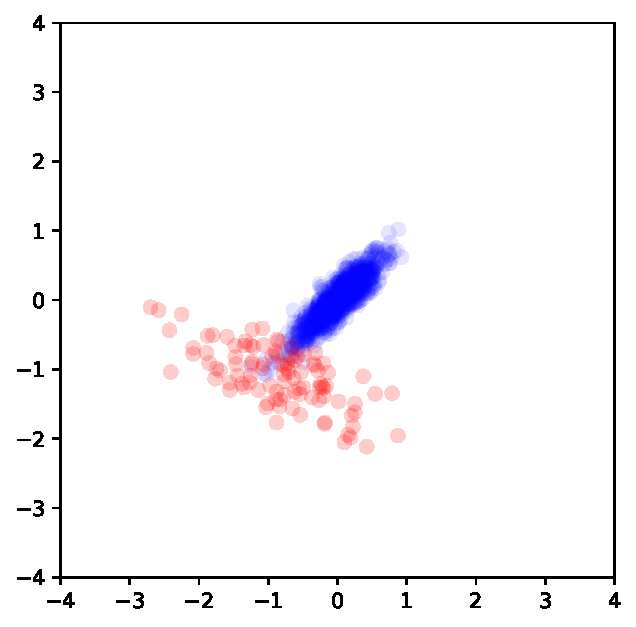
\includegraphics[width=.9\textwidth]{gan1}
        \end{minipage}
        \begin{minipage}{.3\textwidth}
         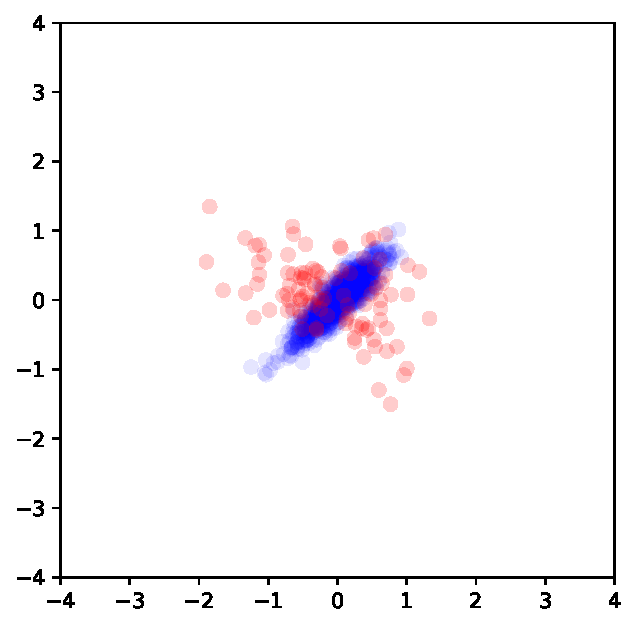
\includegraphics[width=.9\textwidth]{gan2}
        \end{minipage}
        \begin{minipage}{.3\textwidth}
        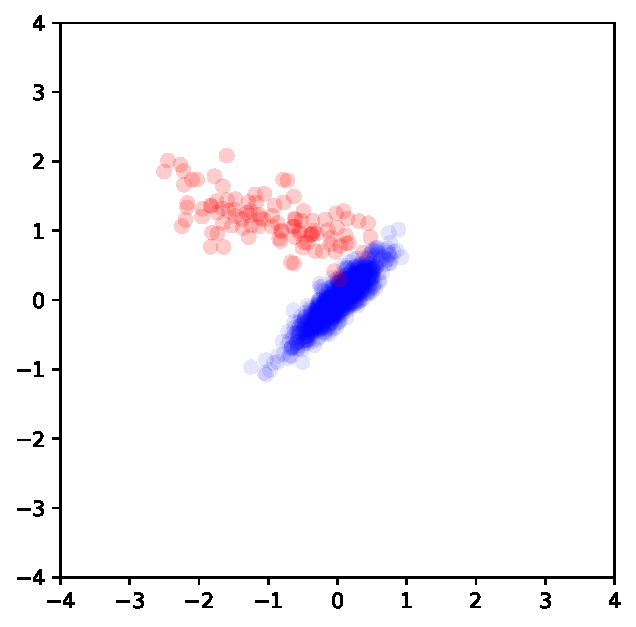
\includegraphics[width=.9\textwidth]{gan3}
        \end{minipage}
        \caption{Snapshots of the evolution with alternating updates}
        \label{fig:gan}
    \end{figure}
    
    \item 
    \begin{align}
        \max_{f \in \mathcal{F}} \E_{\XX\sim \mu}[f(\XX)] - \E_{\YY\sim \nu}[f(\YY)] = \max_{v \in \mathbb{R}^2} \vv^T (\E_{\XX\sim \mu}[\XX] - \E_{\YY\sim \nu}[\YY]) \geq 0
        \label{eq:dist}
    \end{align}
    where the inequality follows by setting $\vv = \0$, which is not necessarily the maximum.
    
    \item In the case that the first moment coincide for both distributions $\mu$ and $\nu$, we have that $\E_{\XX\sim \mu}[\XX] = \E_{\YY\sim \nu}[\YY]$, so \eqref{eq:dist} is satisfied with equality in this case.
    
    This is explains the observed behavior of the GAN since it can estimate the first moment but higher order moments such as the covariance defining the shape of the true distribution. Hence, the obtained distribution keeps oscillating around a zero mean distribution but don't converge to the true one.
    
\end{enumerate}

\subsection*{Problem 2 - Optimizers of Neural Network}

The training accuracy and cross-entropy loss for several optimizers and learning rates can be seen in Figure \ref{fig:optim}, where the mean and variance over three runs is depicted.

\begin{itemize}
    \item \texttt{sgd: }We can see that SGD is the best optimizer for the learning rate of 0.5, but its performance decreases for the lower learning rate of 0.01 and it barely improves with the lowest step size, where we can see that its loss and accuracy remains flat over all the epochs.

    \item \texttt{momentumsgd: }When we add momentum to SGD, we overshoot for large step sizes but get better performance than the naive SGD when the learning rate decreases. This is because the momentum effectively increases the learning rate when the descent direction remains stable in consecutive iterations and thus improves with small learning rates but decreases the performance for large learning rates.
    
    \item \texttt{adagrad: }This optimizer adapts its learning rates for every direction but yet we can observe the influence of the initial step size, specially for the value of $10^{-5}$. It is the best performing optimizer for the step size of 0.01 and its worst performance is attained at the lowest of the tested learning rates.
    
    \item \texttt{rmsprop: }Similarly to AdaGrad, we have adapting learning rate, but in this case, the updates of the effective step size from one iteration to the following one, are in a moving average fashion instead of a simple hard assignment. This is specially beneficial for the learning rate of $10^{-5}$, where we have a rather flat region where AdaGrad slowly converges. Nevertheless, we can see that for a large initial step size, the moving average updates don't allow to rapidly change the effective step size as it happens with AdaGrad.
    
    \item \texttt{adam: }In addition to RMSProp, ADAM uses 2nd order moment estimation. Hence, we observe the same flat behavior for the large step size as RMSProp and as discussed earlier, the momentum doesn't help in this case. With lower learning rates, Adam achieves the best performance since it can adapt its learning rate and further accelerate if the descent direction remains the same from one iteration to another with the momentum term.
\end{itemize}

\begin{figure}
        \centering
        \begin{minipage}{.45\textwidth}
         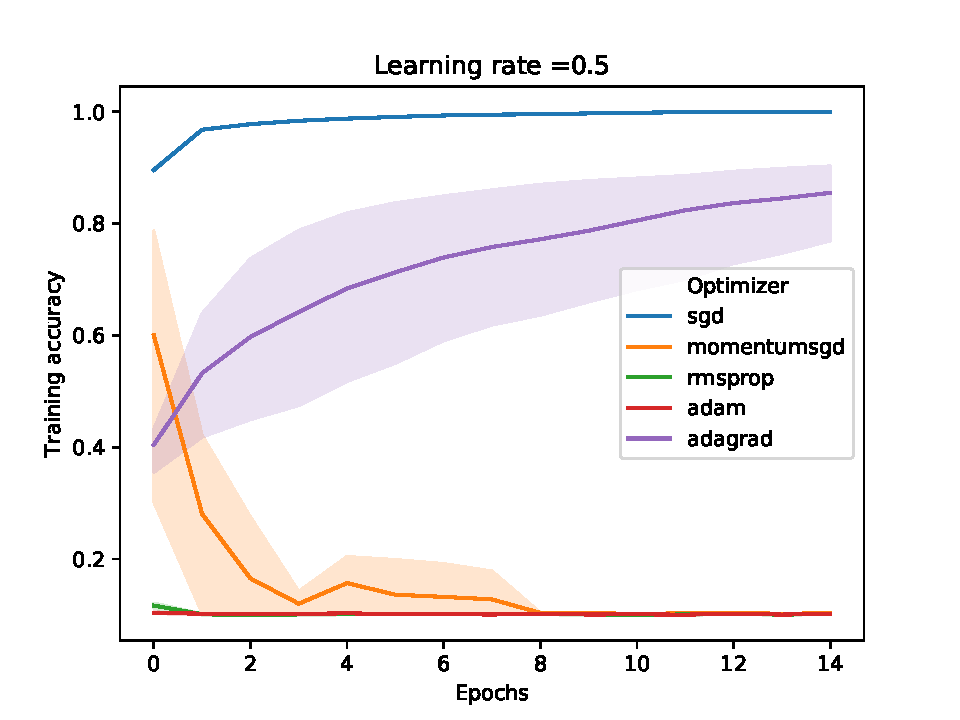
\includegraphics[width=.9\textwidth]{acc_05}
        \end{minipage}
        \begin{minipage}{.45\textwidth}
         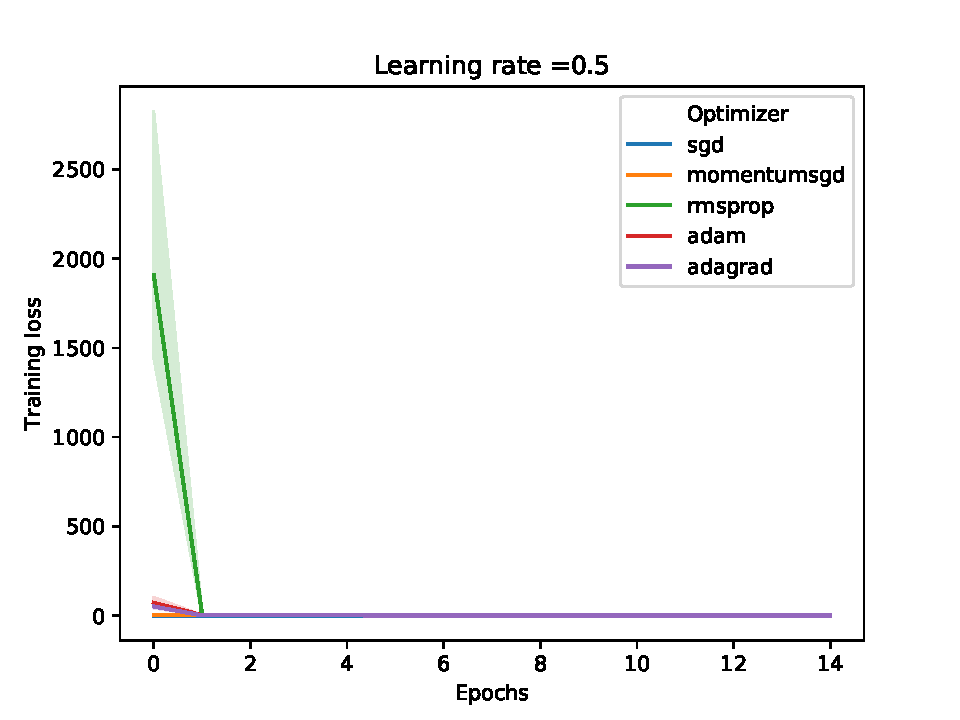
\includegraphics[width=.9\textwidth]{loss_05}
        \end{minipage}
        \begin{minipage}{.45\textwidth}
         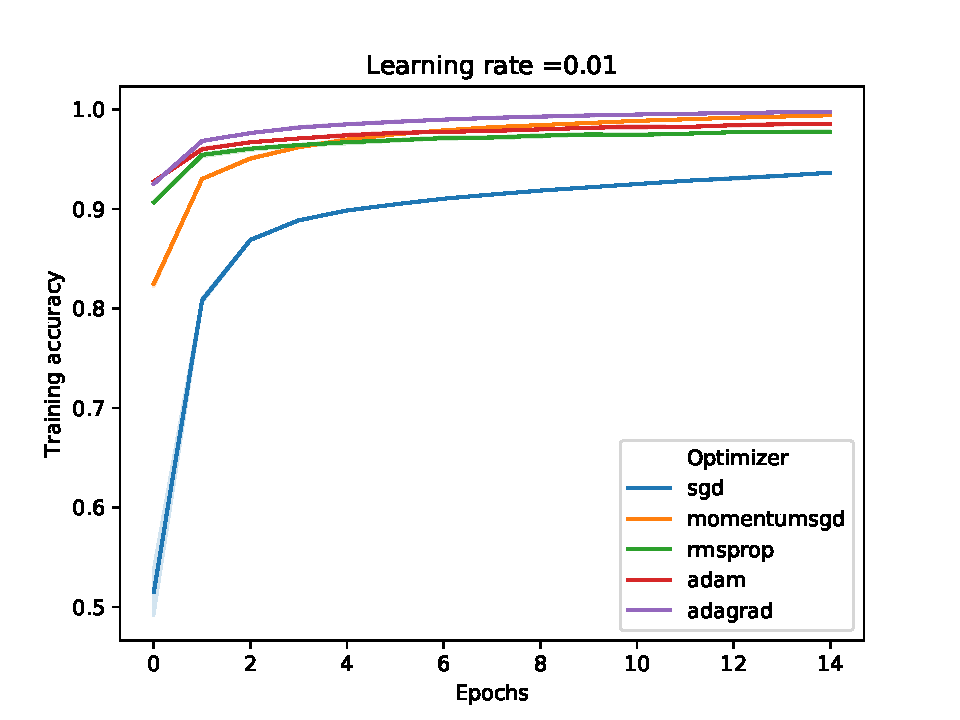
\includegraphics[width=.9\textwidth]{acc_001}
        \end{minipage}
        \begin{minipage}{.45\textwidth}
         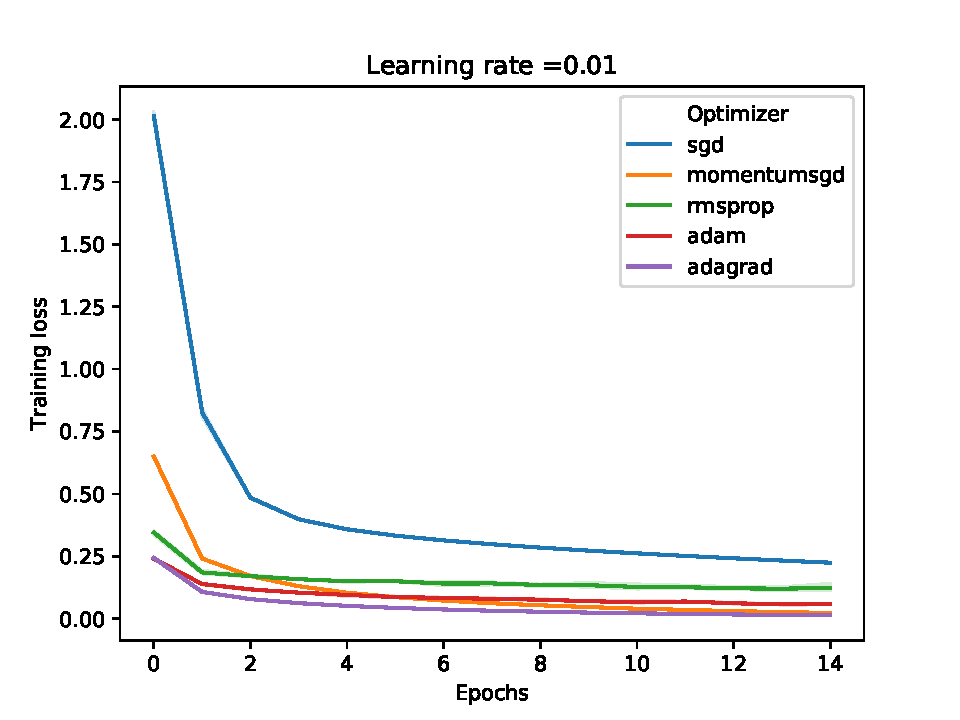
\includegraphics[width=.9\textwidth]{loss_001}
        \end{minipage}
        \begin{minipage}{.45\textwidth}
         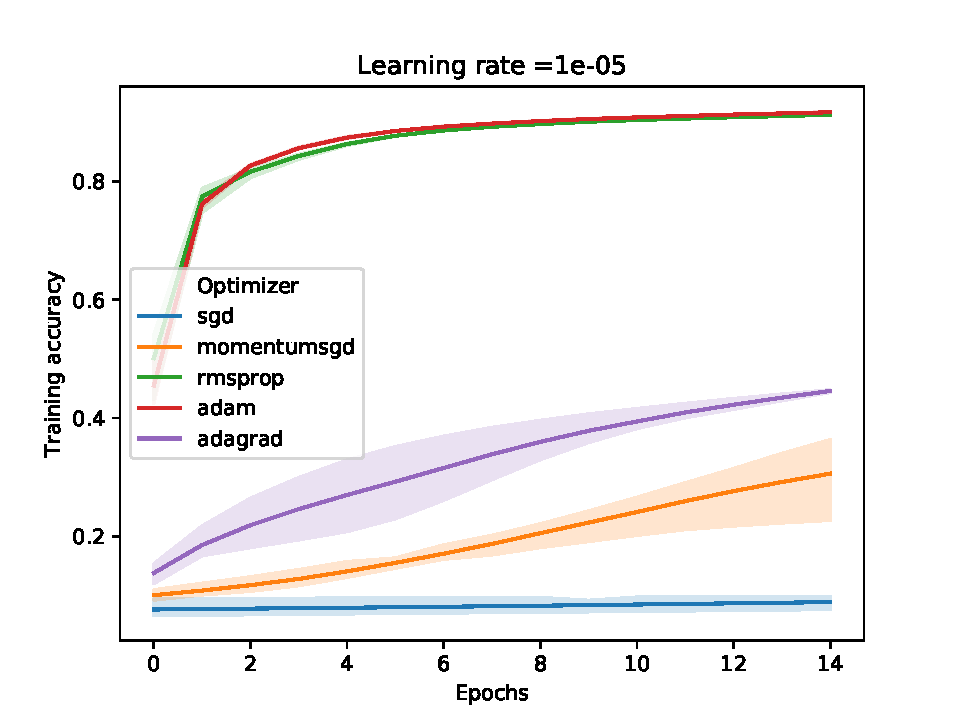
\includegraphics[width=.9\textwidth]{acc_1e-05}
        \end{minipage}
        \begin{minipage}{.45\textwidth}
         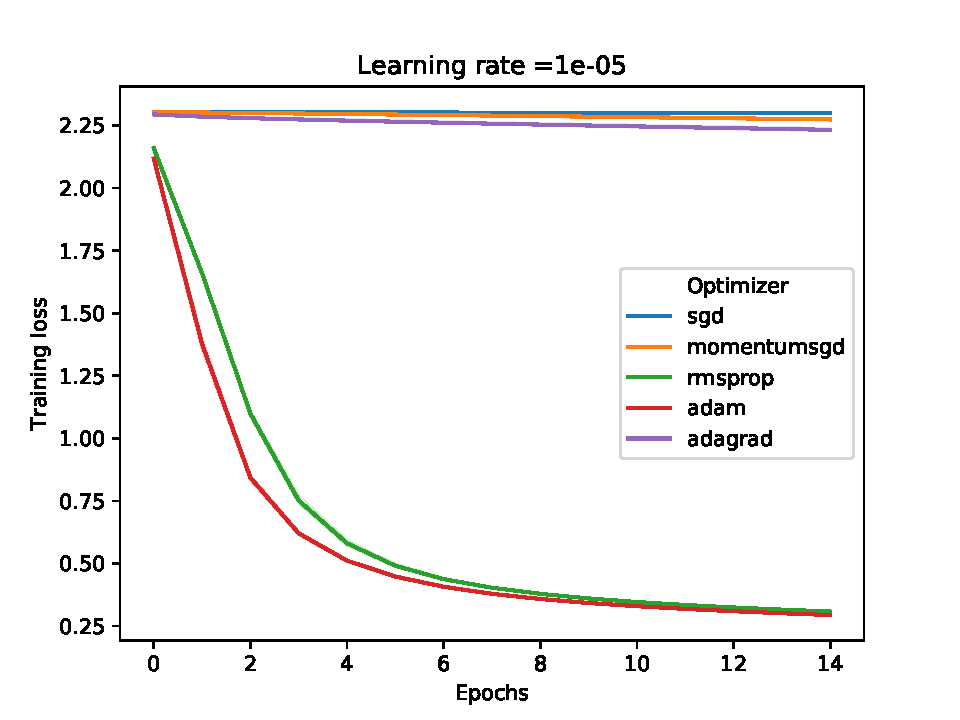
\includegraphics[width=.9\textwidth]{loss_1e-05}
        \end{minipage}
        \caption{Comparison of the implemented optimizers for various learning rates over 3 runs}
        \label{fig:optim}
    \end{figure}

\end{document}
